
\subsection{Overview}
The architecture of the system is composed of two main components: the \ac{eMSP} and the \ac{CPMS}.

\subsubsection{\ac{eMSP} overview}

\begin{figure}[!h]
    \begin{center}
        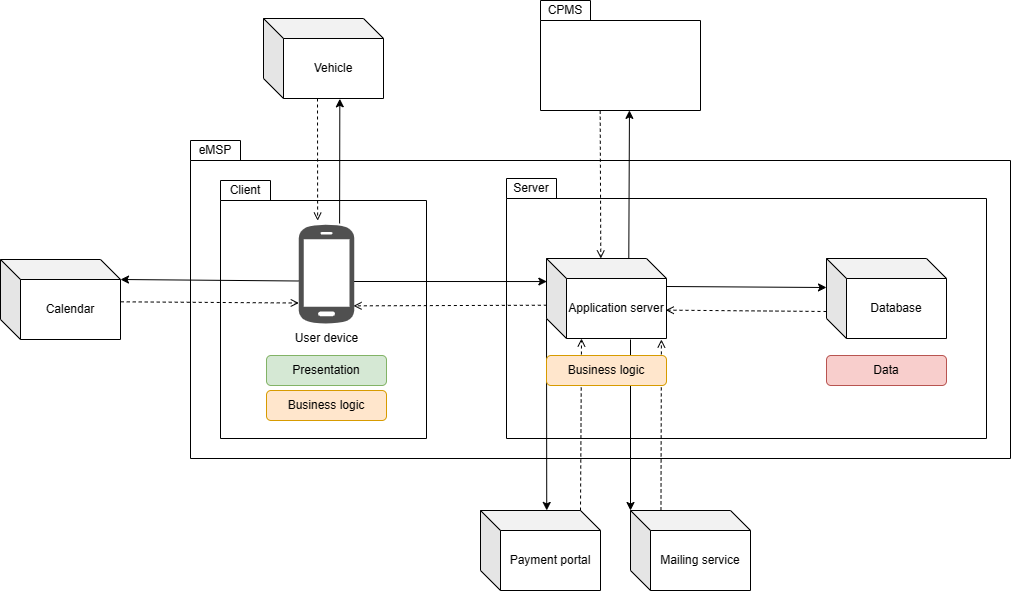
\includegraphics[keepaspectratio, width=0.75\textwidth]{Graphics/DD-eMSP-overview.drawio.png}
        \caption{\ac{eMSP} architectural overview}
        \label{fig:eMSP-overview-architecture}
    \end{center}
\end{figure}

The \ac{eMSP} is a \textbf{three-tier} architecture with \textbf{fat-clients} as seen in \autoref{fig:eMSP-overview-architecture}. This architecture is chosen for different reasons:
\begin{itemize}
    \item Makes the system more scalable;
    \item Allows the separation between business logic and data so that we can apply different levels of dependability to different decoupled systems and we can manage how data is accessed in a more granular way;
    \item There will be a lot of data to be handled in this system (such as booked charges, all the infos about \acp{CPO}, etc.); for this, a dedicated and optimized infrastructure is chosen to be the best choice;
    \item The database will only be accessible by the middleware, constituting an additional layer of security;
    \item With fat-clients the number of messages transmitted are fewer and lighter: an initial elaboration can be done on the smart devices of the user without sending a lot of raw data to the remote application server. The local on-the-edge elaboration is not considered as a problem given the computational power of smartphones.
\end{itemize}
The software pattern applied for this architecture will be the \textbf{\ac{MVC} pattern}. This is the best suit for our application because, being it a web application, we want the components to be as modular, flexible and scalable as possible in order to simplify their distribution.
Also, the separation among view logic and business logic enables us to turn the client application in a fat one, moving the whole view logic in the client application. \todo{ha senso come commento?}

The following paragraphs will describe the principal components of this pattern and their architectural distribution.

\paragraph{Model}
The model is the logical representation of the persistent data. This is stored in a database system and will only be directly accessible by the server application.

\paragraph{View}
The view logic will be completely delegated to the client application, representing in different ways the data retrieved from the model.

\paragraph{Controller}
The controller will have to manage all the client requests, interacting with the model, modifying it and returning to the view the changed/retrieved data.
In our application, for the most part, the business logic will be in the server application. Just the part of retrieving and processing the vehicle data and the calendar appointments (in the case of a request for smart suggestions of the application) will be handled by the client application so that the communication with the application server will be as simple as possible.

\subsubsection{\ac{CPMS} overview}

\begin{figure}[!h]
    \begin{center}
        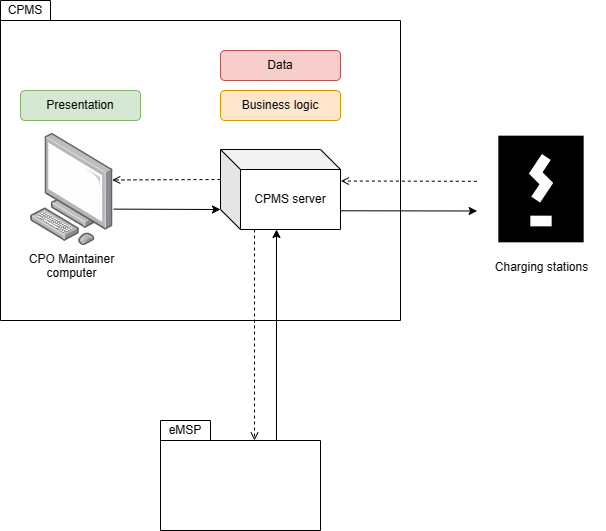
\includegraphics[keepaspectratio, width=0.75\textwidth]{Graphics/DD-CPMS-overview.drawio.png}
        \caption{\ac{CPMS} architectural overview}
        \label{fig:CPMS-overview-architecture}
    \end{center}
\end{figure}

The \ac{CPMS} follows the \textbf{two-tier} pattern with \textbf{thin-clients} as seen in \autoref{fig:CPMS-overview-architecture}. This architecture is chosen for different reasons:
\begin{itemize}
    \item The system is simpler to implement with respect to the three-tier architecture;
    \item The system shouldn't handle so much data, so it isn't necessary to have a dedicated architecture for the data layer;
    \item Clients are thin because they only have to view infos about charging stations and can send simple events (for example \textit{use \ac{DSO} X for charging station Y}, \textit{set revenue percentage to Z}, etc.).
\end{itemize}
Also for this system we will use the \ac{MVC} pattern. In this case, the client will only have the view logic and can send simple events. All the elaboration, the management of the \acp{DSO} and activation/deactivation of charging process of batteries are handled by the \ac{CPMS} server, which handles the business logic and the data.
The \ac{CPMS} server, on the other hand, will deal also with charging requests from \acp{eMSP}, to which it will respond with the elaborated data.


\subsection{Component view}
\begin{figure}[!h]
    \begin{center}
        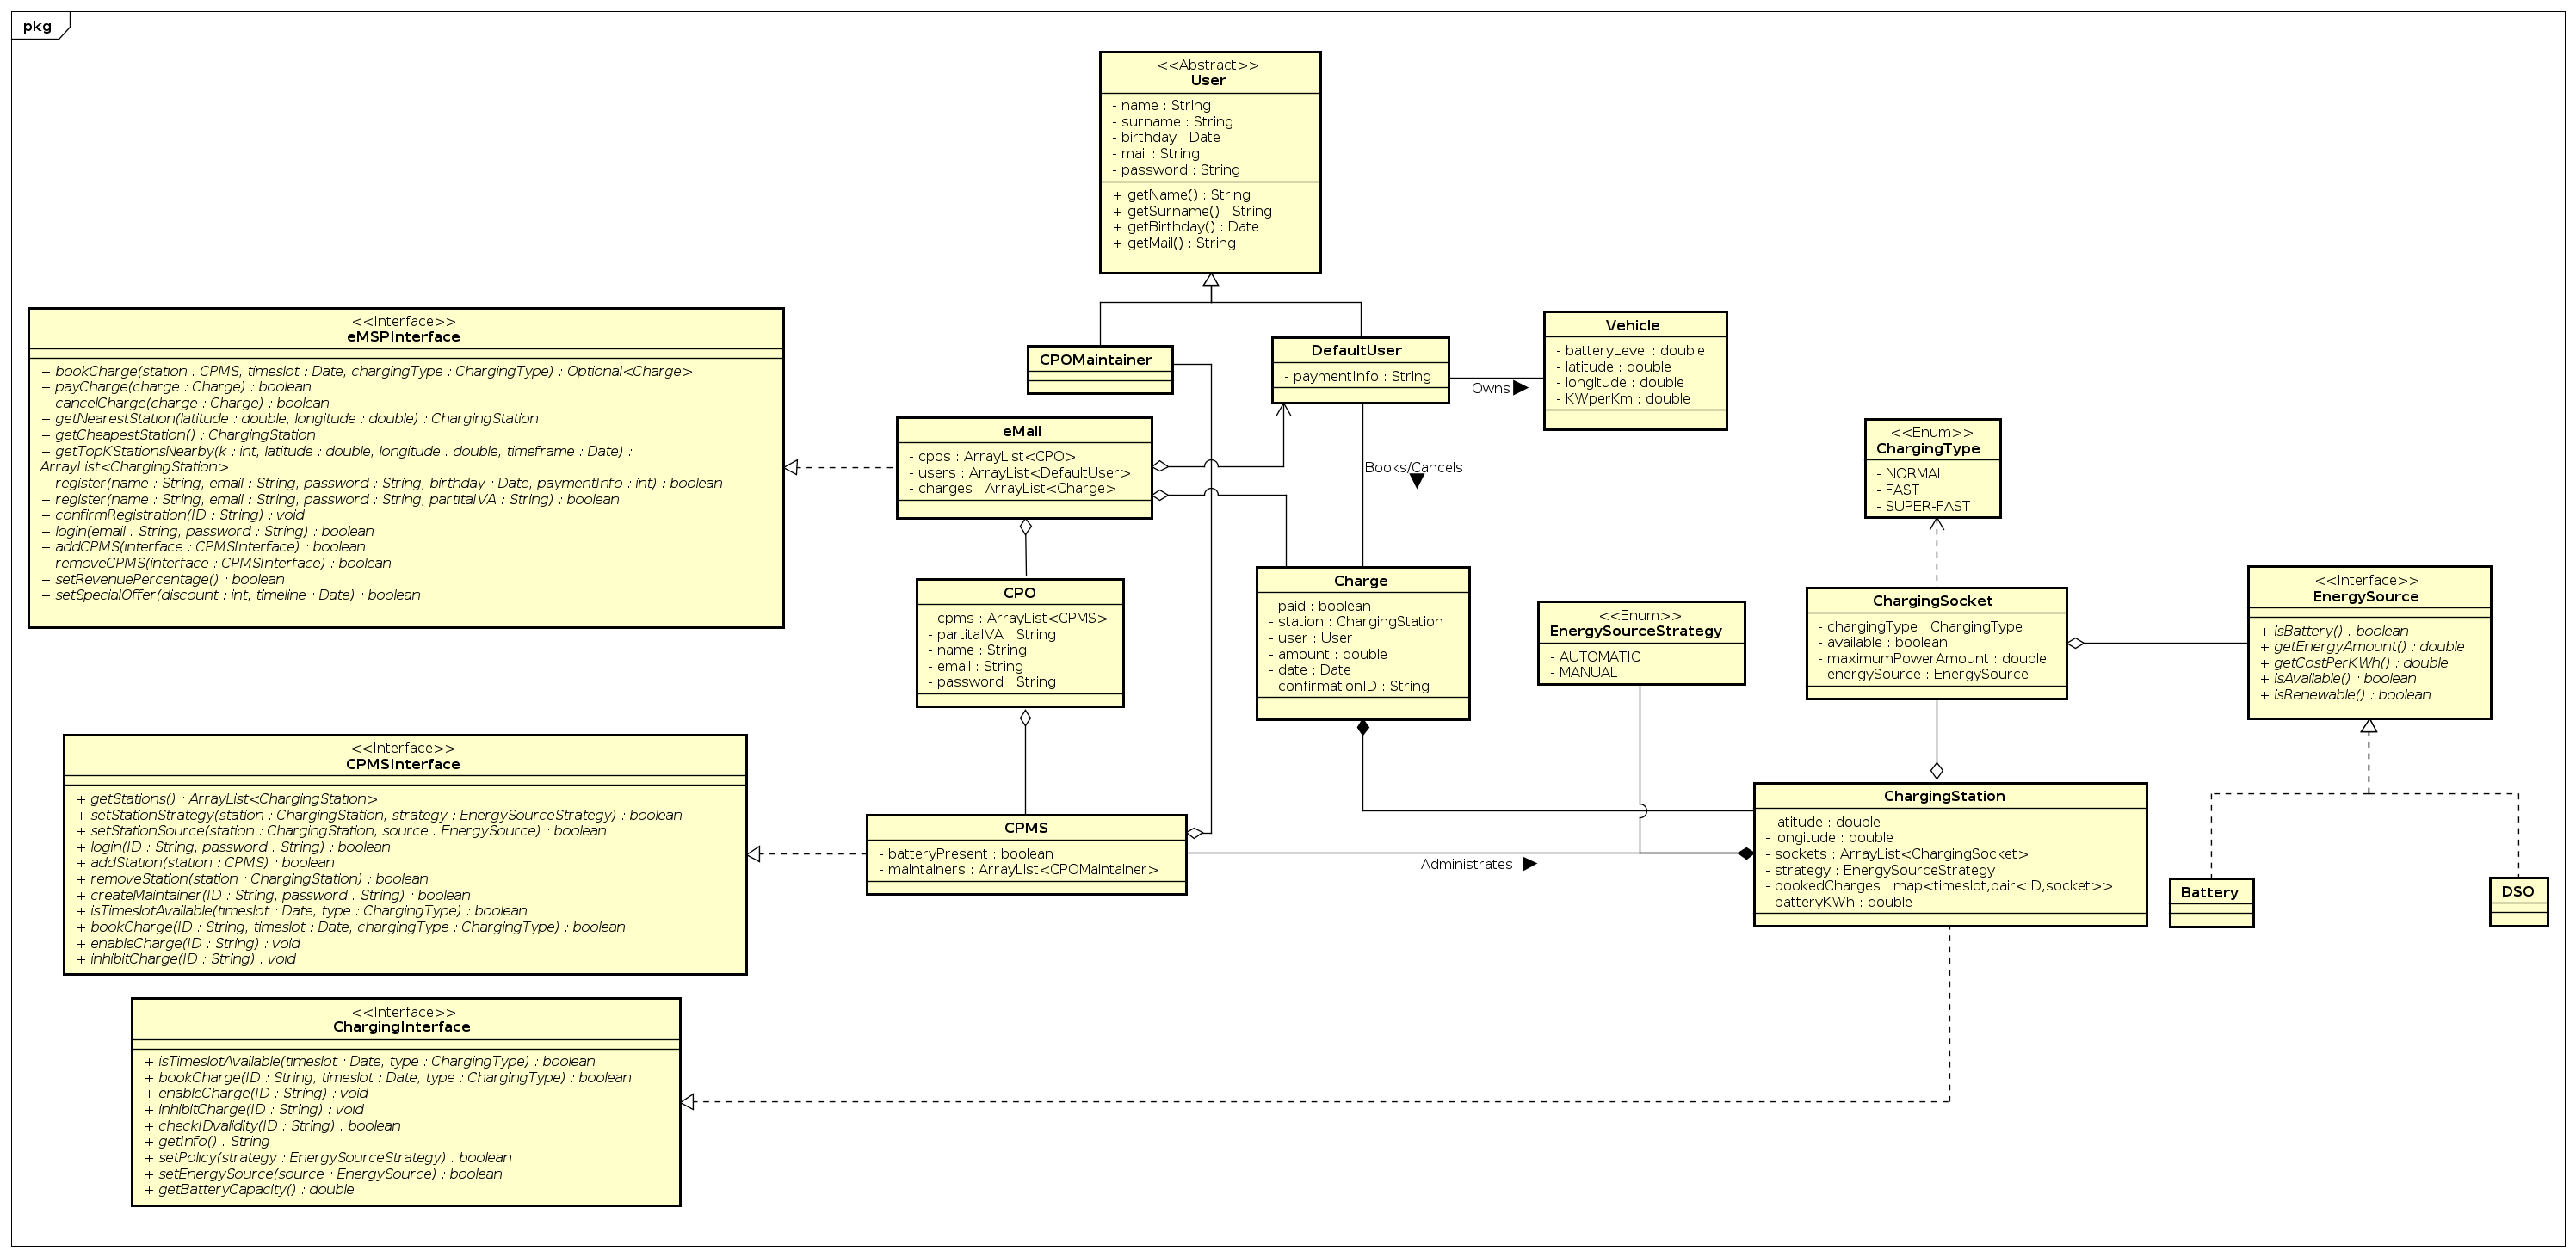
\includegraphics[keepaspectratio, width=16cm]{UML.png}
        \caption{Class diagram}
        \label{fig:UML}
    \end{center}
\end{figure}
In the class diagram illustrated in \autoref{fig:UML} a model (not functional) view of the system is represented. The \ac{eMall} and \ac{CPMS} interfaces show what the two systems are expected to implement, whereas for the ChargingInterface it is assumed an already existing implementation.

\subsubsection{Component diagrams}
\begin{figure}[!h]
    \begin{center}
        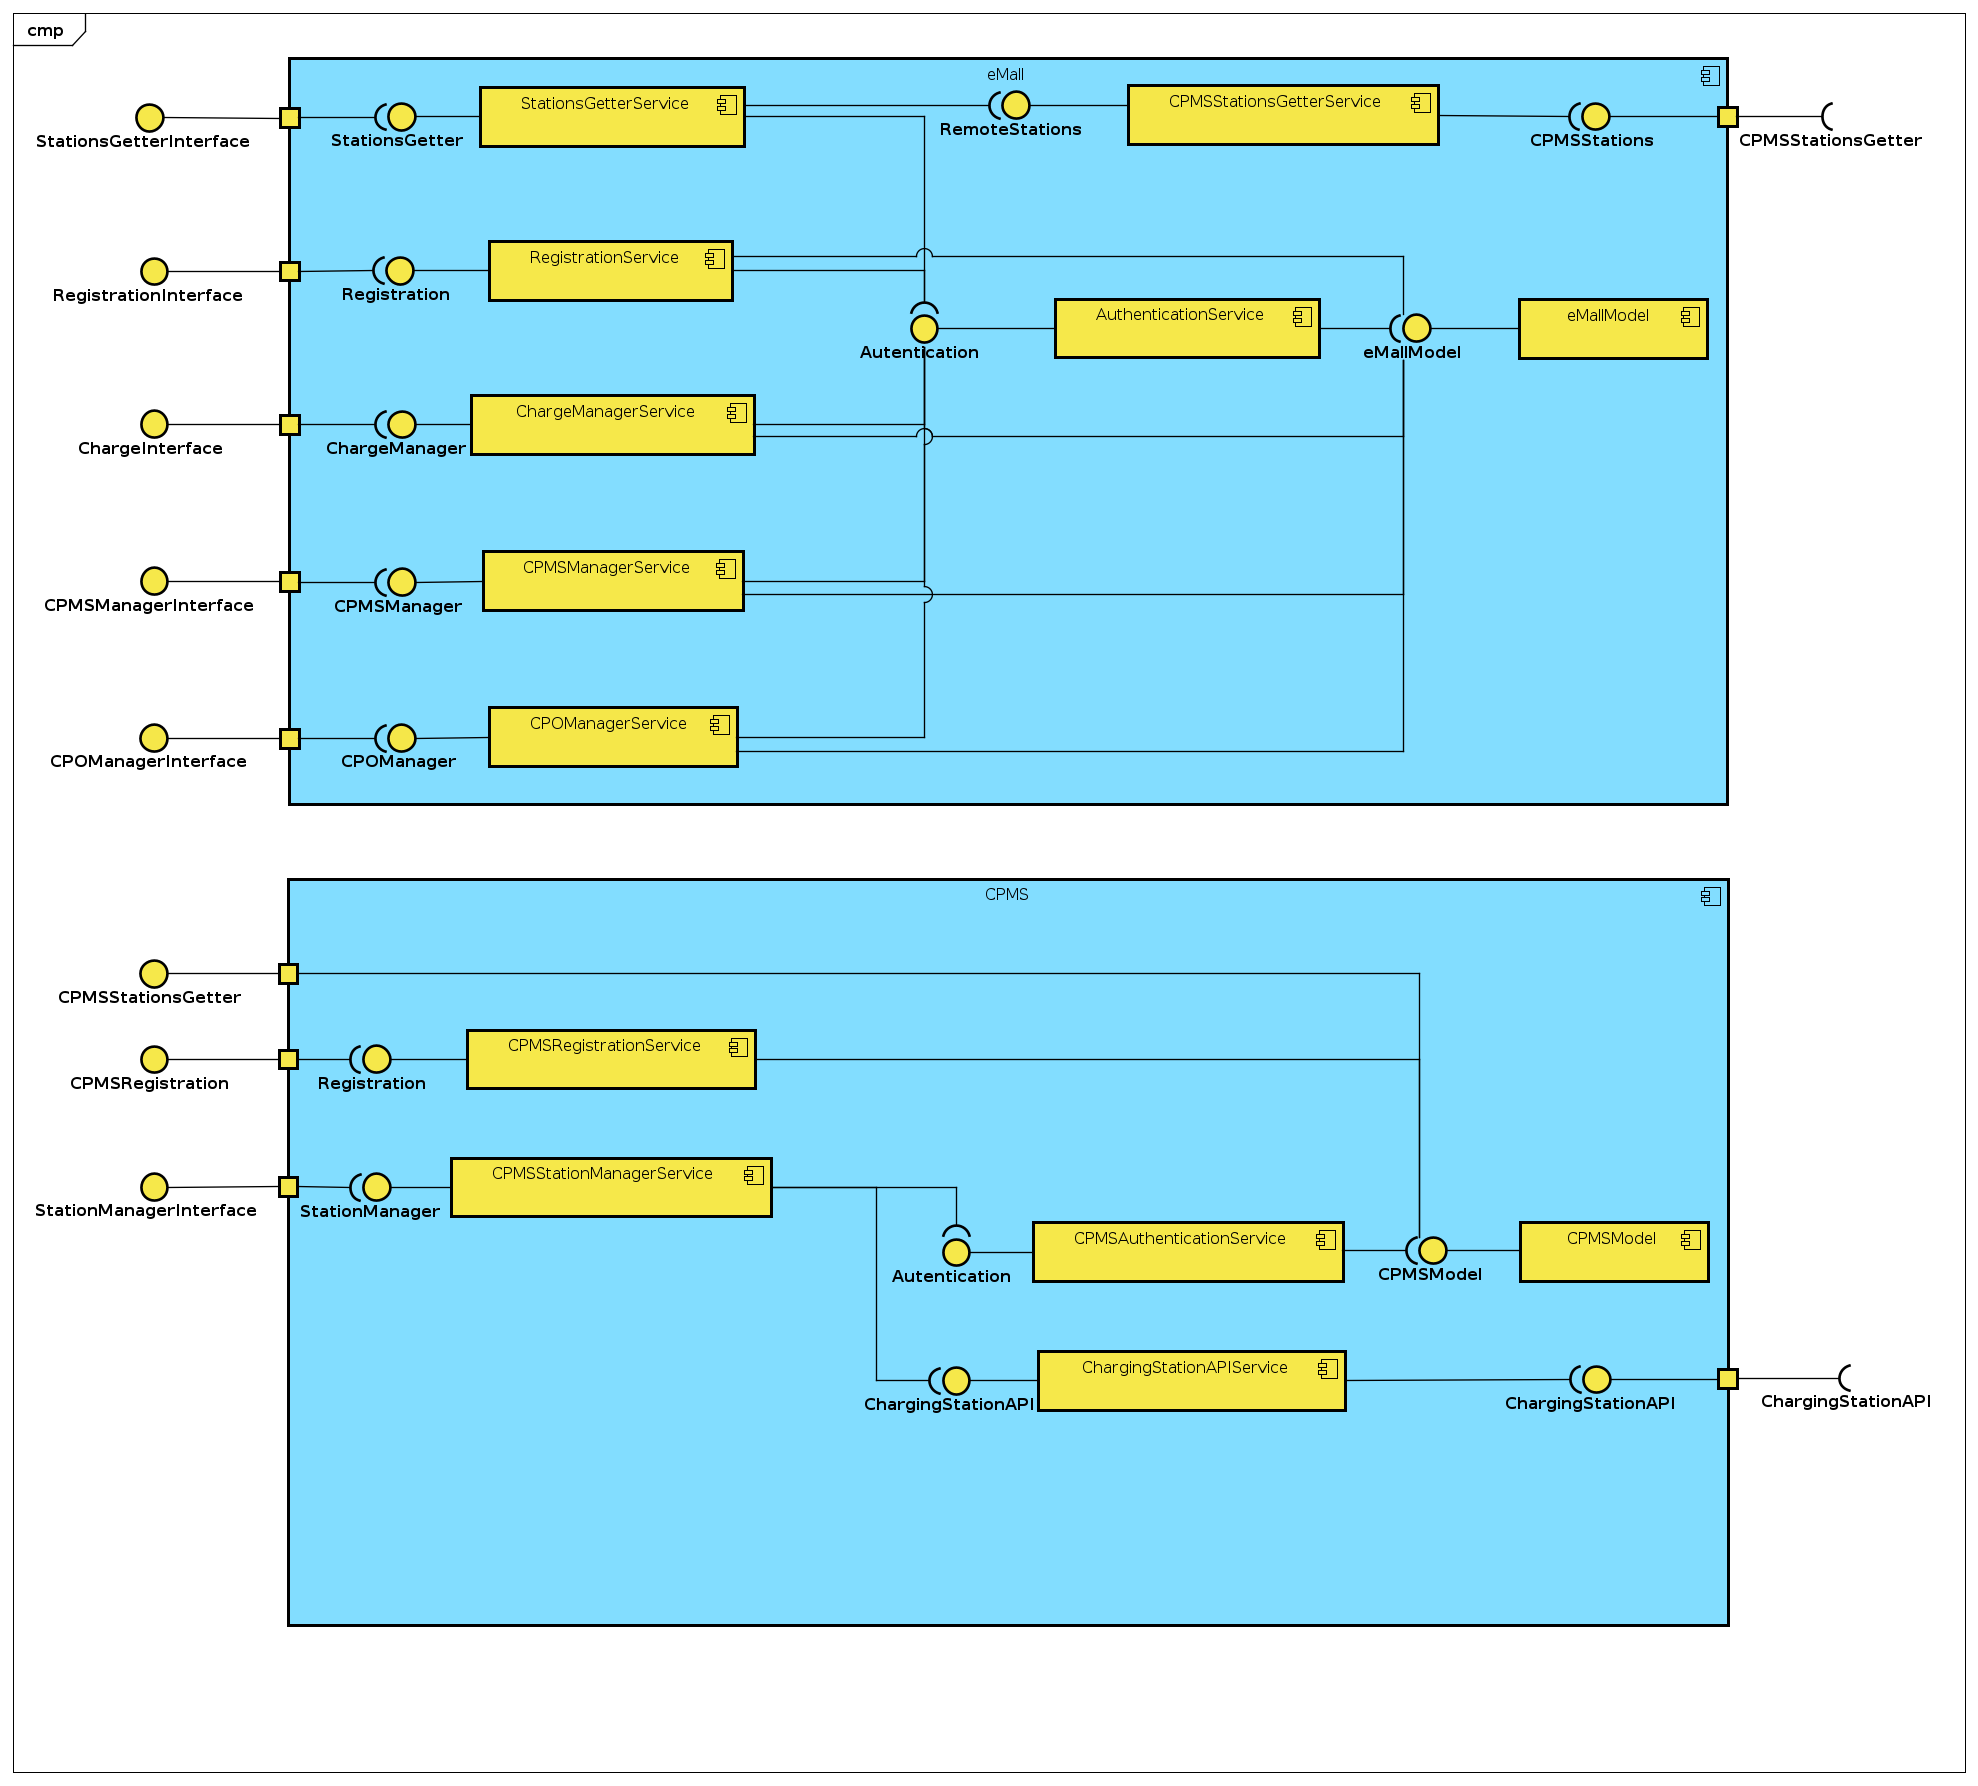
\includegraphics[keepaspectratio, width=16cm]{Component/Component.png}
        \caption{eMall component diagram}
        \label{fig:eMSP-component}
    \end{center}
\end{figure}
\clearpage
The two systems implement different interfaces and represent the \textit{Controller} and \textit{Model} parts of the \ac{MVC} pattern.

\paragraph{\textbf{\ac{eMall}}}
The main components for the \ac{eMall} system are:
\begin{itemize}
    \item \textbf{StationsService}: It is the component responsible for handling all the stations research requests (like \textit{getNearestStations}, \textit{getCheapestStation}, \textit{getTopKStationsNearby});
    \item \textbf{RegistrationService}: It is the component responsible for handling the registration details along with the parameters checking during the registration phase;
    \item \textbf{ChargeManagerService}: It is the component responsible for handling all the charge booking/payment/cancellation processes. It interfaces with the payment \ac{API} and with the charging station \ac{API};
    \item \textbf{\ac{CPMS}ManagerService}: It is the component responsible for handling the \ac{CPMS} operations from the \acp{CPO} users;
    \item \textbf{\ac{CPO}ManagerService}: It is the component responsible for handling the \acp{CPO} requests (like \textit{SetRevenuePercentage} and \textit{setSpecialOffer});
    \item \textbf{\ac{CPMS}StationsService}: It is the component responsible for providing the list of charging stations from the \ac{CPMS};
    \item \textbf{AuthenticationService}: It is the component responsible for authorizing every operation over the model component. At this level it is implemented part of the controller (of the \ac{MVC} pattern) to check that operation is legit for the account type;
    \item \textbf{Payment \ac{API}}: It is a component that interfaces the \ac{eMall} system with the external payment \acp{API};
    \item \textbf{ChargingStation \ac{API}}: It is a component that interfaces the \ac{eMall} system with the charging stations \acp{API}. Without this component, operations like \textit{bookCharge}, \textit{enableCharge} and \textit{inhibitCharge} couldn't be done;
    \item \textbf{\ac{eMall}Model}: It is the core component. It stores all the \ac{eMall} data and interfaces them with the other system components.
\end{itemize}
There are some apparently similar components, but there are some slight differences:
\begin{itemize}
    \item The \ac{CPO}ManagerService is conceptually different from the \ac{CPMS}ManagerService because the CPMS manager service alters the stations collection of the model according to the interface with the inserted \ac{CPMS};
    \item The \ac{CPMS} StationsService is different from the ChargingStation \ac{API} because the \ac{CPMS} StationService interfaces with the inserted \acp{CPMS} and the ChargingStation \ac{API} interfaces the \ac{eMall} with the charging stations to handle the charge booking/enabling and canceling features.
\end{itemize}
\paragraph{\textbf{\ac{CPMS}}}
The main components for the \ac{CPMS} system are:
\begin{itemize}
    \item \textbf{\ac{CPMS}RegistrationService}:
    \item \textbf{\ac{CPMS}StationManager}:
    \item \textbf{\ac{CPMS}AuthenticationService}:
    \item \textbf{ChargingStation \ac{API}}:
    \item \textbf{\ac{CPMS}Model}:
\end{itemize}

\subsection{Deployment view}
\subsubsection{\ac{eMSP}}
\begin{figure}[!h]
    \begin{center}
        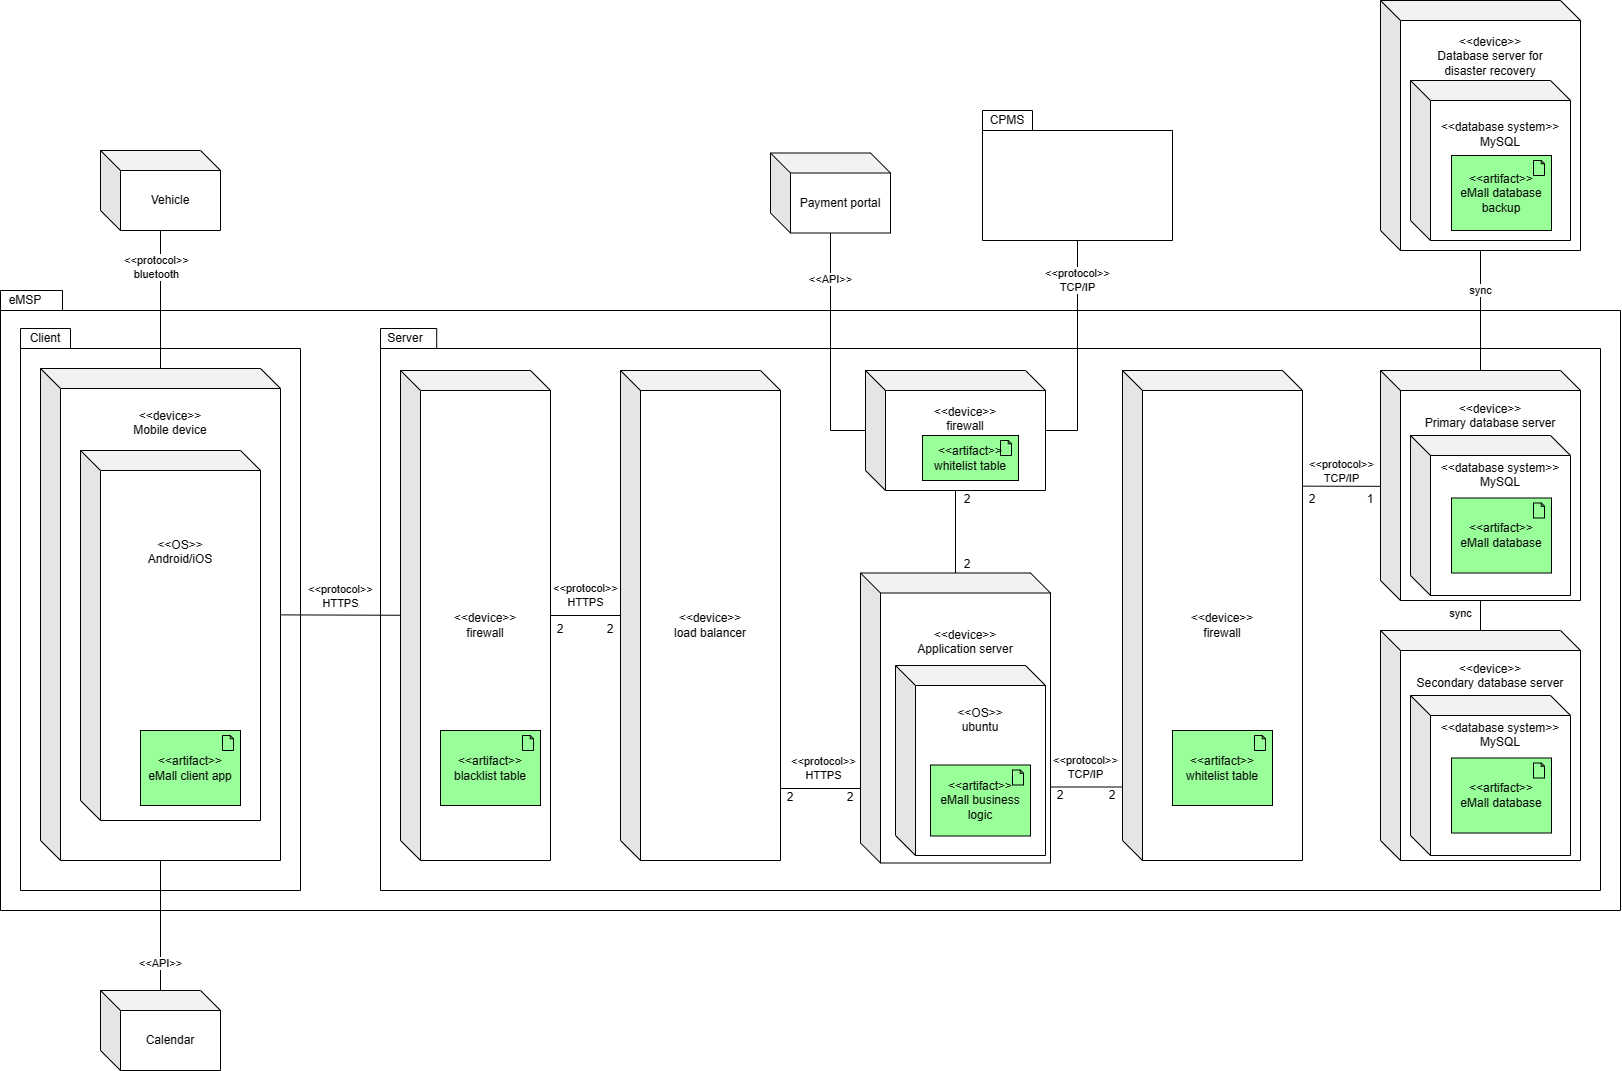
\includegraphics[keepaspectratio, width=0.9\textwidth]{Graphics/DD-eMSP-deployment.drawio.png}
        \caption{eMall deployment view diagram}
        \label{fig:eMSP-deployment}
    \end{center}
\end{figure}

\begin{itemize}
    \item protocol application server - CPMS
    \item protocol user device - server
    \item 1 load balancer
    \item 2 application servers
    \item disaster recovery DB
\end{itemize}

\subsubsection{\ac{CPMS}}
\begin{figure}[!h]
    \begin{center}
        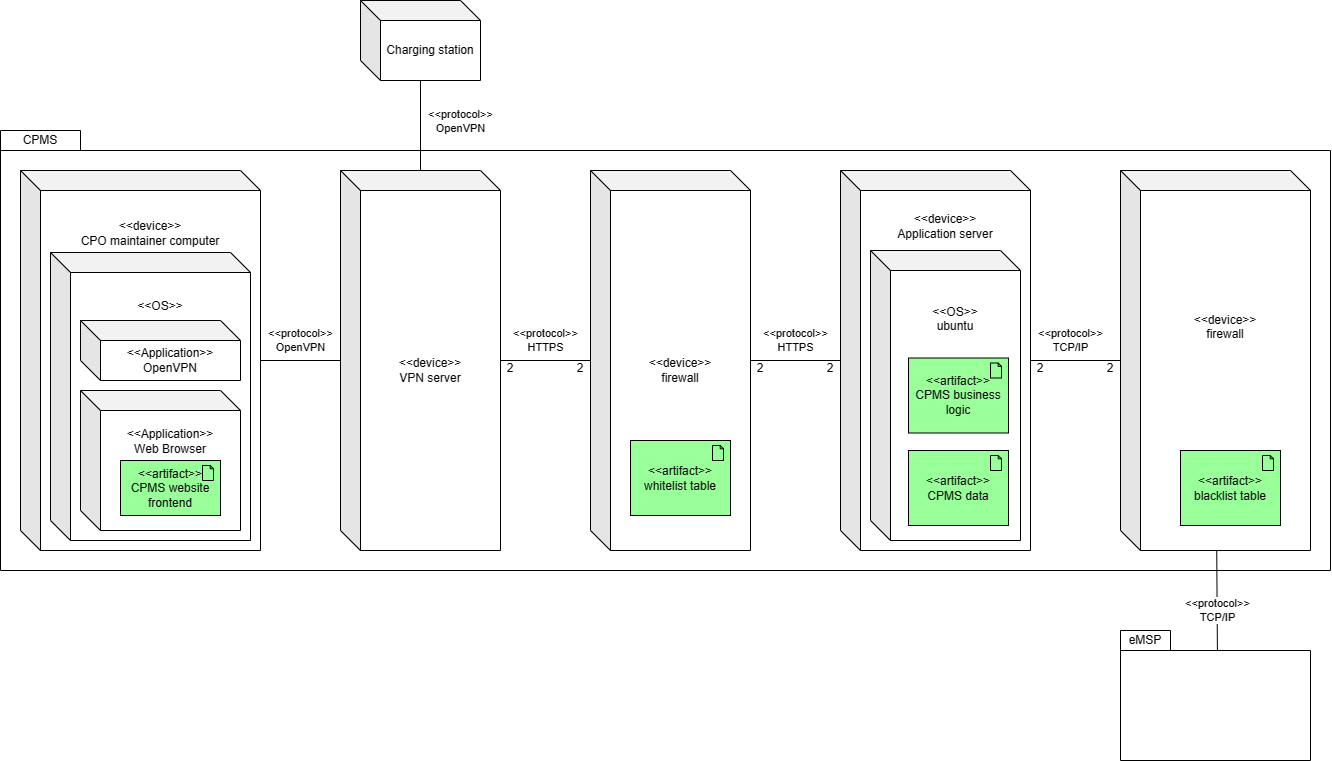
\includegraphics[keepaspectratio, width=0.9\textwidth]{Graphics/DD-CPMS-deployment.drawio.png}
        \caption{CPMS deployment view diagram}
        \label{fig:CPMS-deployment}
    \end{center}
\end{figure}

\begin{itemize}
    \item protocol eMSP - application server
    \item protocol CPO maintainer - application server
\end{itemize}
\clearpage

\subsection{Runtime view}
\subsection{Component interfaces}
\subsection{Selected architectural styles and patterns}
\subsection{Other design decisions}
\clearpage